\section{Hoe is het algoritme tot stand gekomen?}
Na assessment 1 was de doelstelling voor assessment 2, het autonoom laten rijden van de \gls{Smart-Car}. Hier is de projectgroep Infra Vroom dan ook aan begonnen. 
\subsection{Zelf rijd algoritme}
Er is gestart met het uitdenken van een flowchart voor het autonoom laten rijden van de \gls{Smart-Car} terwijl het obstakels ontwijkt. Dit werd stap voor stap gedaan. Iedere stap werd vervolgens omgezet tot code en getest. Als dit werkte werd de volgende stap gezet, werkte dit niet, dan werd er naar een oplossing gezocht. 

\begin{figure}[h]
    \centering
    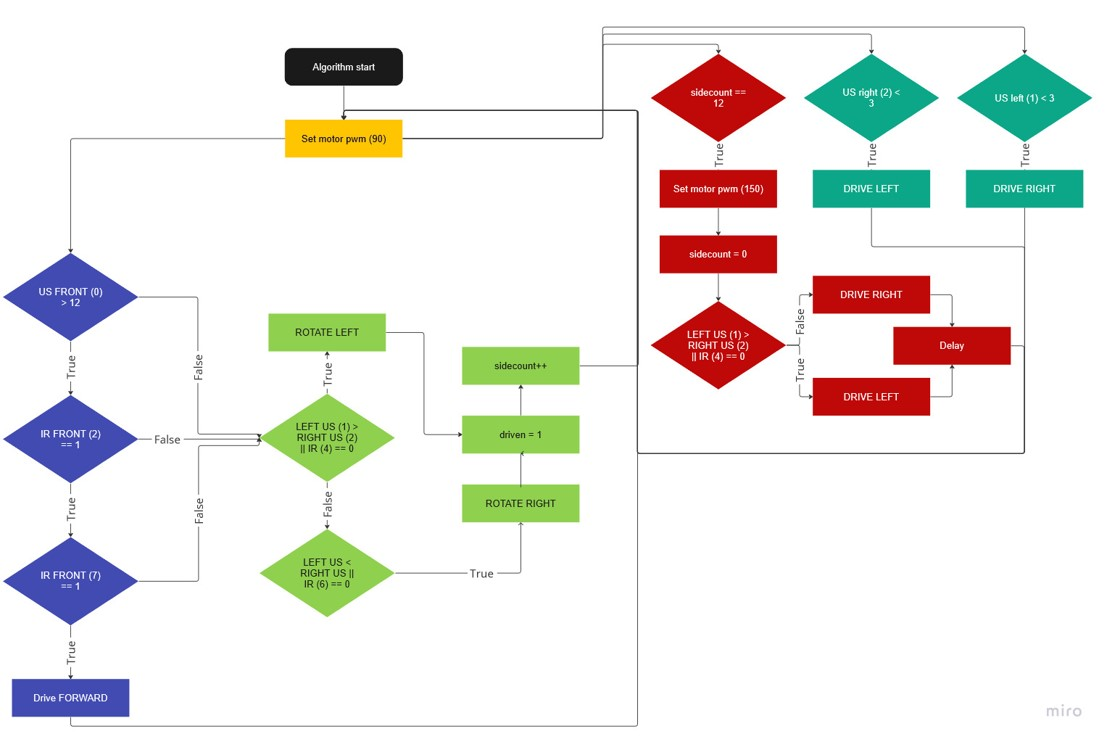
\includegraphics[scale = 0.59]{Media/Figuren/zelf rijd algoritme.jpg}
    \caption{Basis zelf rijd en obstakel vermijding algoritme}
    \label{Zelf rijd algoritme}
\end{figure}

De eerste stap was de \gls{Smart-Car} vooruit laten rijden zolang het aan de voorkant geen obstakel detecteerde. Dit was vrij snel uitgedacht in een flowchart, omgezet tot code en werkend getest. (donkerblauwe gedeelte figuur \ref{Zelf rijd algoritme})

De volgende stap was het uitdenken wat de \gls{Smart-Car} moet doen als het wel een obstakel voor zich ziet. Er is besloten in dit geval de zijwaarts gerichte ultrasoon sensoren te gebruiken om te bepalen aan welke kant meer ruimte is. De \gls{Smart-Car} controleert of aan de kant waar meer ruimte is, genoeg ruimte is om heen te draaien. (lichtgroene gedeelte figuur \ref{Zelf rijd algoritme}) Als dit het geval is draait hij daarheen, als niet, is de situatie dat de \gls{Smart-Car} is ingesloten door drie muren aan voor- en beide zijkanten. In dat geval moet stap drie uitgevoerd worden. 

Stap drie is het algoritme dat de \gls{Smart-Car} uit deze situatie krijgt. Uit testen bleek dat de \gls{Smart-Car} in deze situatie heen en weer blijft roteren omdat het telkens tijdens het draaien aan de andere kant een grotere afstand meet. Daarom is stap drie hierop aangepast. Deze wordt nu uitgevoerd zodra de \gls{Smart-Car} twaalf keer in korte successie heen en weer draait / probeert te draaien. De \gls{Smart-Car} zal dan nog één keer kijken aan welke zijkant meer ruimte is en vervolgens die kant op zijwaarts rijden. Vervolgens zal de \gls{Smart-Car} weer vanaf het begin het algoritme uitvoeren. 

Naast deze stappen is er ook een gedeelte van het algoritme (turquoise gedeelte figuur \ref{Zelf rijd algoritme}) dat ervoor zorgt dat de \gls{Smart-Car} kort zijwaarts wegrijdt van een obstakel als deze te dichtbij de zijkant van de \gls{Smart-Car} is. 

Dit is het algoritme dat voor de demonstratie van assessment 2 gebruikt is (zie figuur \ref{Zelf rijd algoritme} voor de code). In het kort zorgde dit algoritme ervoor dat de \gls{Smart-Car} autonoom obstakels kon ontwijken en beslissingen kon maken over welke kant hij op moest gaan. 

\subsection{Toevoeging periscoop algoritme met servo}
Na assessment 2 is de periscoop geleverd. Met deze periscoop was de doelstelling, het kunnen vinden en detecteren van een laser zuil. Hiervoor zou de periscoop op een servo bevestigd worden en zou er een algoritme voor moeten worden geschreven die de periscoop laat zoeken naar het laser zuil. Dit is wederom gedaan door het algoritme stap voor stap uit te denken en hiervoor een flowchart te maken. Tijdens het ontwikkelen van dit algoritme werd de periscoop getest en bleek deze niet accuraat te kunnen meten. Daarom is er besloten de flowchart niet om te zetten in code tot de periscoop werkende is en de code tussentijds ook getest zou kunnen worden. 

Het uitgedachte algoritme met flowchart voor de periscoop met servo was als volgt (figuur 13). 
\begin{figure}[h]
    \centering
    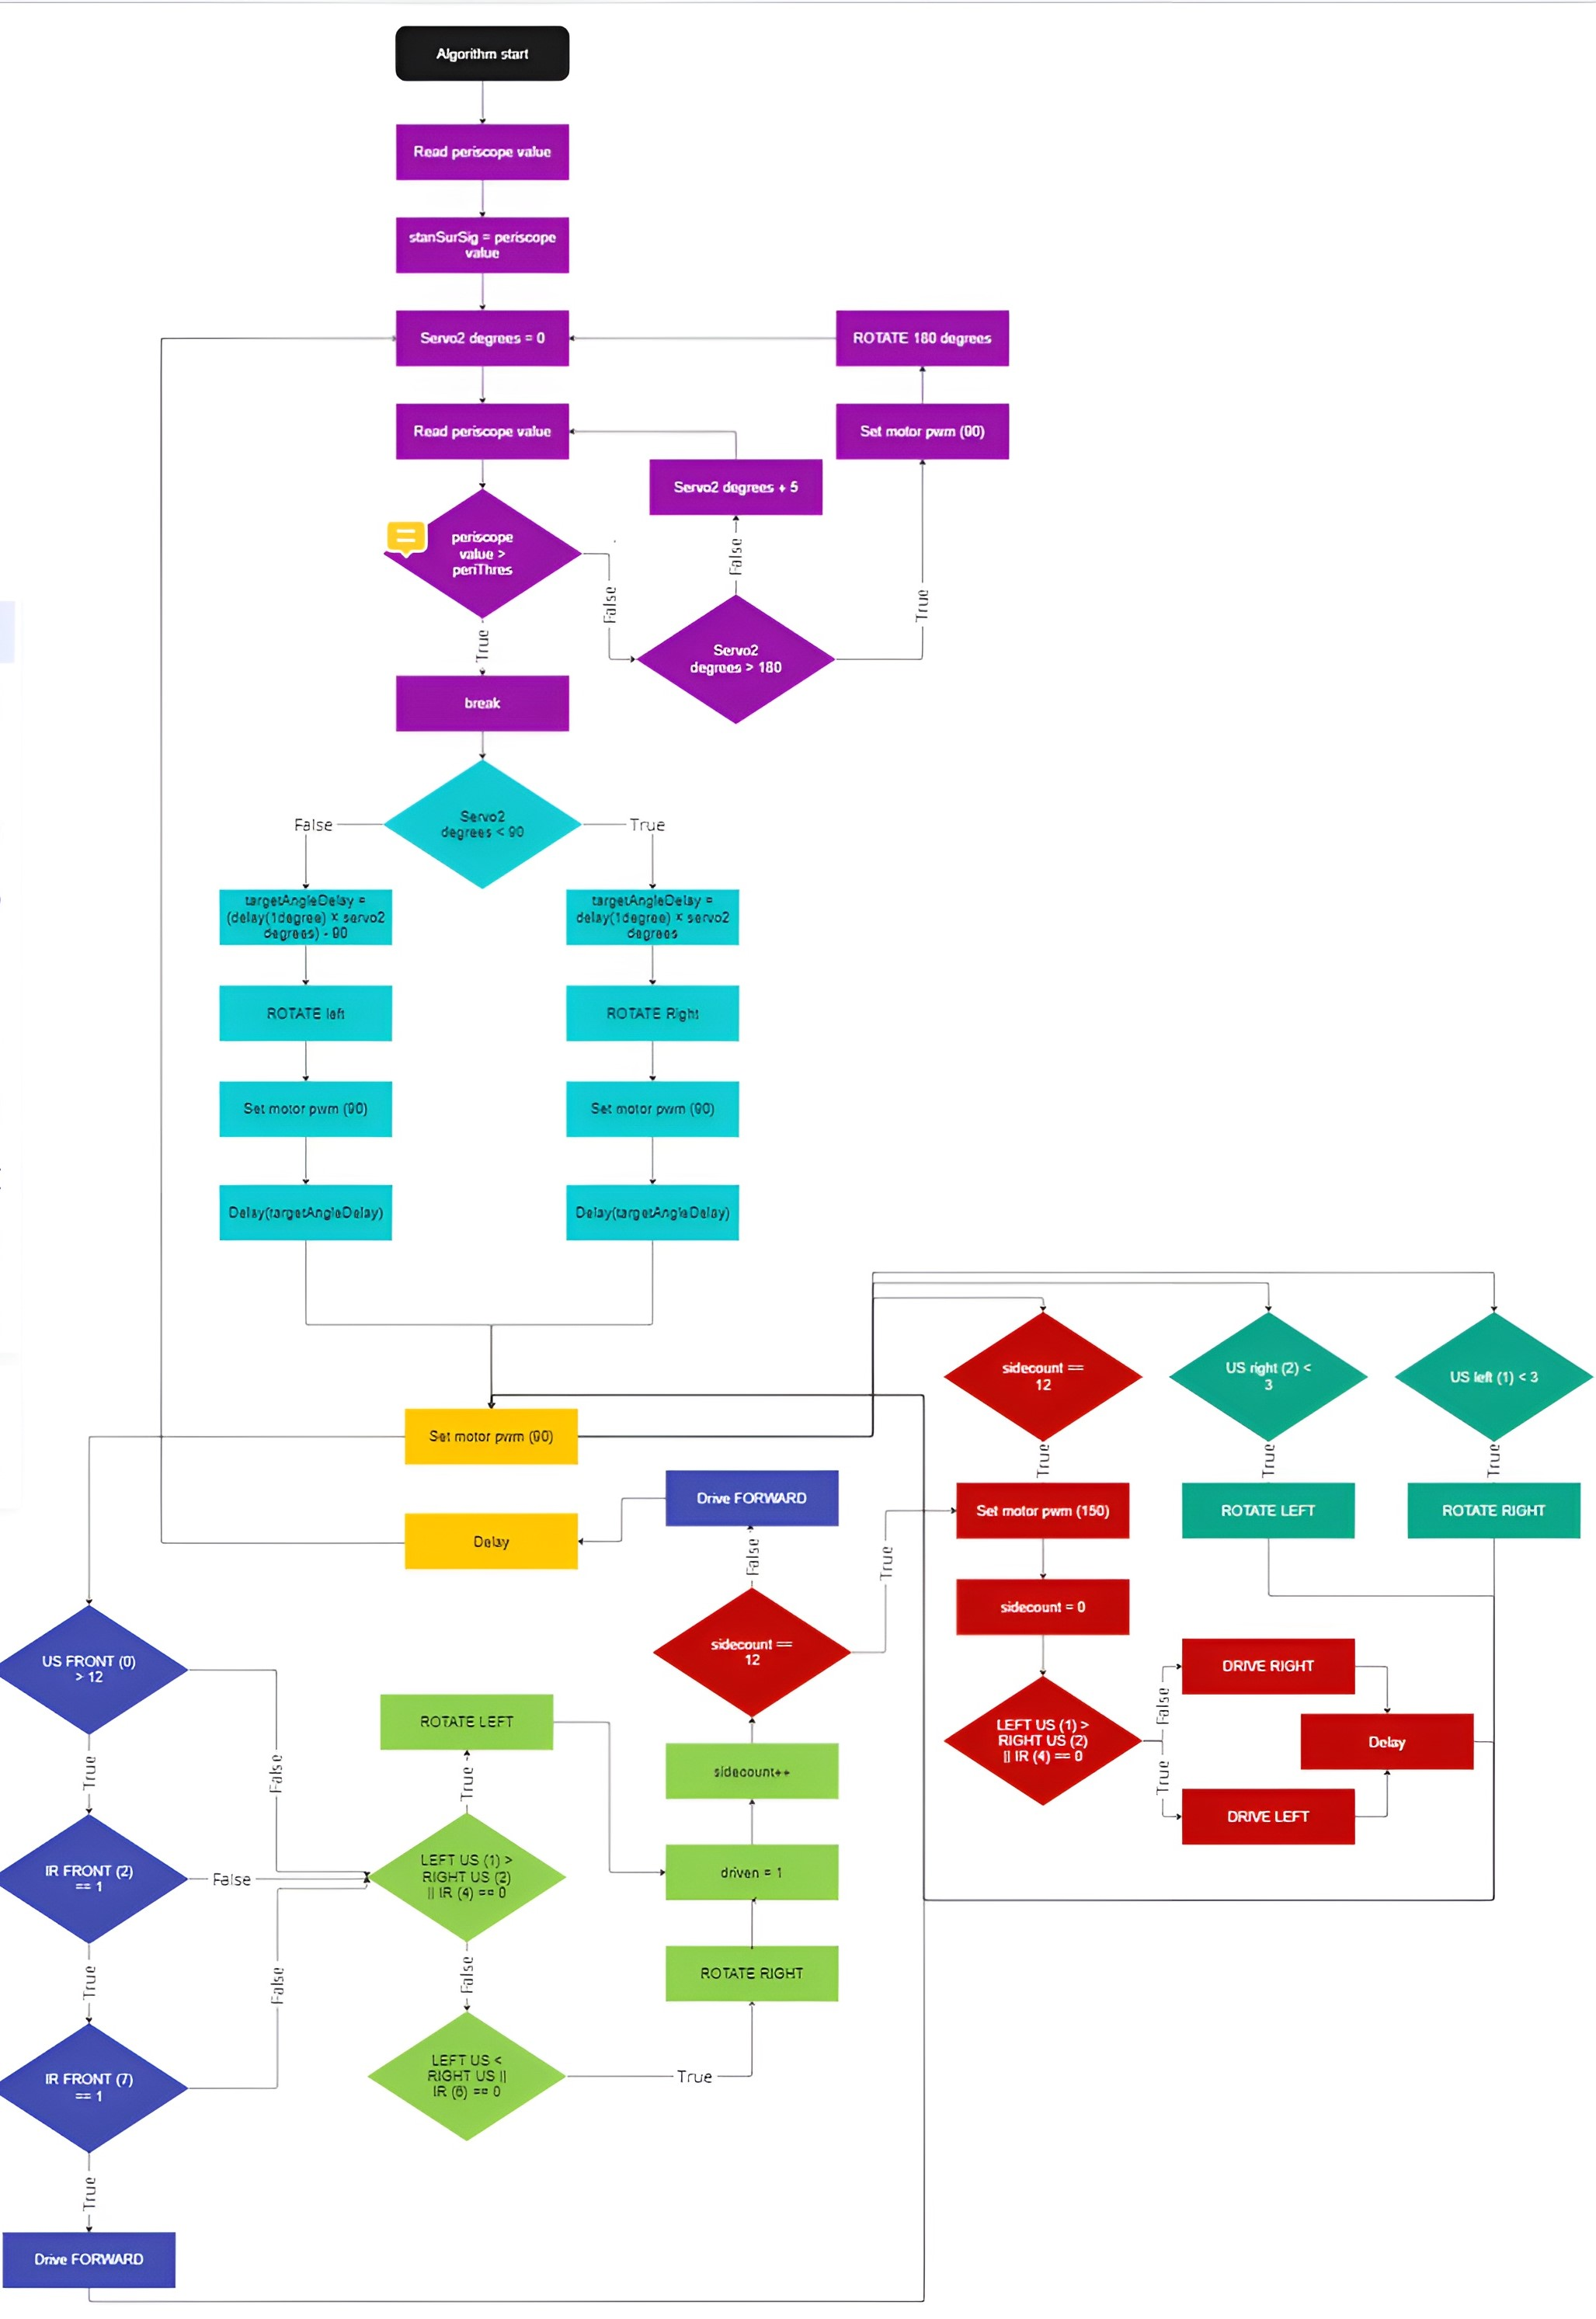
\includegraphics[scale = 0.3]{Media/Figuren/Periscoop algoritme met servo.jpg}
    \caption{Gehele algoritme inclusief periscoop met servo}
    \label{Volledig algoritme met periscoop en servo}
\end{figure}

De \gls{Smart-Car} begint nu niet gelijk met rijden. In plaats daarvan begint hij met het kalibreren van de periscoop zodat deze werkt, onafhankelijk van het omgevingslicht. Vervolgens zal de servo met periscoop erop draaien tot het de gewenste meetwaarde meet. Deze meetwaarde is de waarde die getest zou worden als zijnde die van het laser zuil. Afhankelijk van testen zou dit met een extra marge kunnen worden bepaald. Als de waarde gemeten is, zal door middel van een vooraf bepaalde delay en het aantal graden dat de servo gedraaid is, de nieuwe delay worden bepaald. Deze delay laat de auto draaien naar de richting van de servo (en dus waar het laser zuil zich bevindt). Vervolgens zal het het basisalgoritme met obstakeldetectie weer gaan uitvoeren, waarbij tussentijds telkens opnieuw gescand wordt om er zeker van te zijn dat de \gls{Smart-Car} de juiste richting in rijdt. 
\clearpage
\newpage
\subsection{Toevoeging periscoop algoritme zonder servo}
In een poging de periscoop minder te laten trillen, is de periscoop vastgezet op de \gls{Smart-Car} zelf in plaats van op de hiervoor in eerste instantie bedoelde servo. Dit bleek achteraf te leiden tot een simpeler algoritme. Dit algoritme is wederom uitgedacht en tot flowchart gemaakt. Ook dit algoritme is niet tot code omgevormd, met dezelfde reden als voorheen. De flowchart ziet er als volgt uit (figuur 14).

\begin{figure}[h]
    \centering
    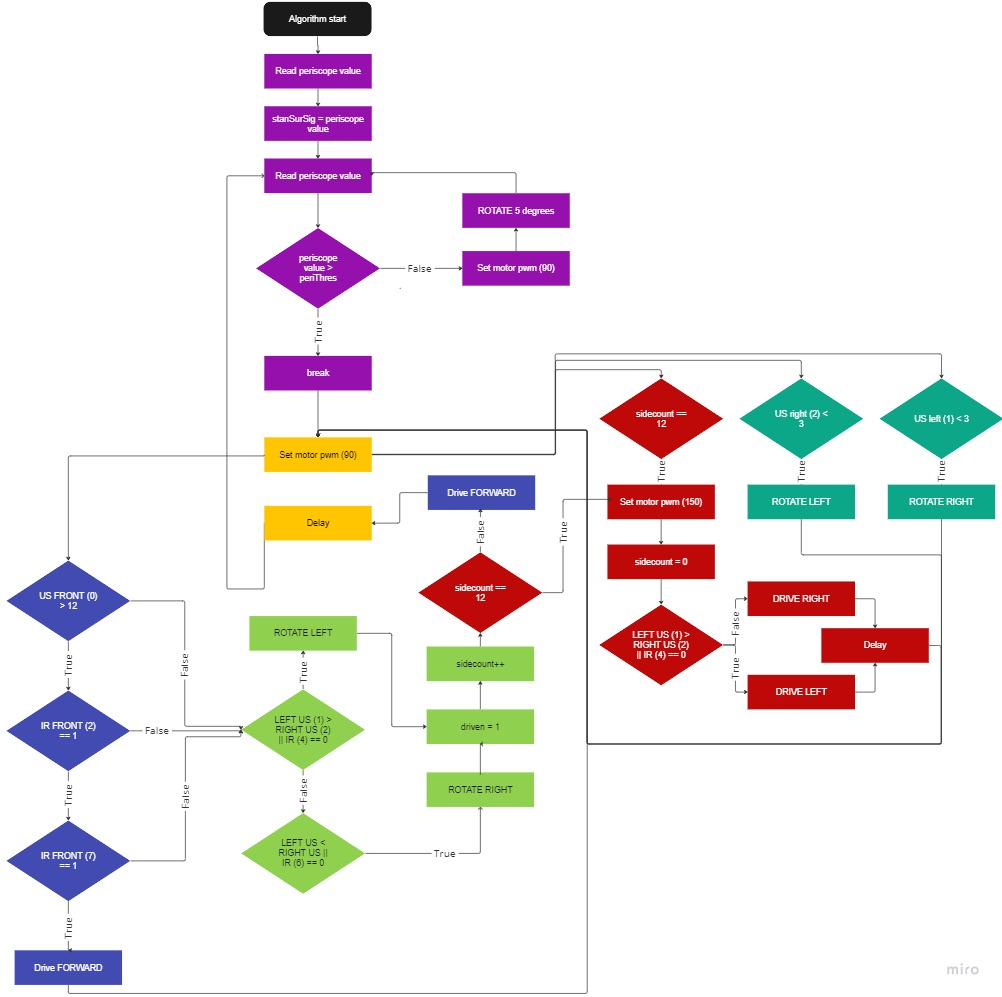
\includegraphics[scale = 0.5]{Media/Figuren/Periscoop algoritme zonder servo.jpg}
    \caption{Gehele algoritme inclusief periscoop zonder servo}
    \label{Volledig algoritme met periscoop, zonder servo}
\end{figure}

Dit algoritme begint hetzelfde als degene met servo. Bij het scannen van de omgeving gebruikt het echter niet de servo, maar draait de volledige \gls{Smart-Car}. Dit zorgt ervoor dat zodra de gewenste meetwaarde gemeten wordt door de periscoop, de \gls{Smart-Car} al de goede kant op gericht is. Hierdoor is het gedeelte van het algoritme dat de richting van de servo bepaald hier niet nodig is. Dit maakt dit algoritme simpeler en voor nu (met deze microcontroller) superieur.